\documentclass[journal]{IEEEtran}
\usepackage{lmodern}
\usepackage{amsfonts}
%\usepackage{hyperref}

\usepackage{cite}
\ifCLASSINFOpdf
  \usepackage[pdftex]{graphicx}
  \graphicspath{{./img/}}
  \DeclareGraphicsExtensions{.pdf,.jpeg,.png}
\else
\fi
\usepackage{array}
\usepackage{url}
\hyphenation{op-tical net-works semi-conduc-tor av-er-age at-tribute}


\begin{document}
\title{Analysis of Genetic Algorithms Optimizing Topological Layout and Synaptic Weights }

\author{Taras~Mychaskiw(xxxxxxx)~\textless{}tm07qx@brocku.ca\textgreater\\%
Evan~Verworn~(4582938)~\textless{}ev09qz@brocku.ca\textgreater% <-this % stops a space
}

\maketitle

\begin{abstract}ah Blah Blah Blah Blah Blah Blah.
\end{abstract}

\IEEEpeerreviewmaketitle

\section{Introduction}
\IEEEPARstart{T}{his} should be written last. Blah Blah Blah Blah Blah Blah Blah Blah Blah Blah Blah Blah Blah. 

\section{Background}

% I don't think we'd have to write much on this and GAs. 
% I think about the same as a wikipedia summary.
  \subsection{Neural Networks}
  A high level description of a basic Neural Network is a single directional graph without cycles or reflexive edges. It is a mathematical model wherein given some number of inputs and some number of outputs, the outputs will react to the magnitude of the input values. A visualization is given in Figure \ref{fig:NeuralNetwork}.
  
\begin{figure}[here]%[!t]
  \centering
  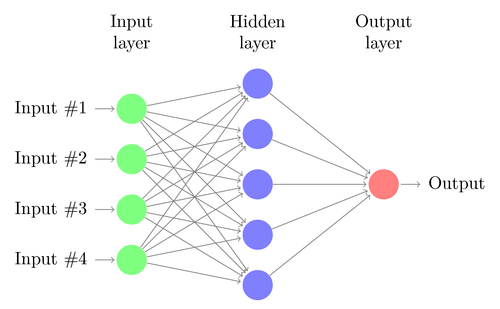
\includegraphics[width=3.4in]{neural-network}
  \caption{An example single hidden layer neural network.}
  \label{fig:NeuralNetwork}
\end{figure}

The output is \textit{trained} to the desired output through manipulating the weights in the intermediate (hidden) and output layer edges.  

\begin{figure}[here]
  \[  node\_output = \sum_{i=1}^{n} w_{i} x_{i} \]
  \caption{Where $n$ is the number of edges coming \textit{into} this node, $w$ is the weight associated with that edge and x is the output value produced by the predecessor node.}
  \label{fig:NodeOutput}
\end{figure}

A node calculates its output value by summing the output of all of its predecessors and multiplying that output by a weight assigned to that edge, this value is then squashed to a number traditionally between 0 and 1 by a Sigmoid function.

In the Figure \ref{fig:NeuralNetwork} there is only one hidden layer, but in our experiments we are evolving a network that can have up to three hidden layers. 

% Talk about backprop.

  \subsection{Genetic Algorithms}
  Genetic Algorithms or GAs are another mathematical model for finding an optimized solution in a large search space. This model is based off of Darwinian Evolution in that the best performing current solutions are bred together mixing genetic information from both parents into their children (known as a crossover operation). These children are then evaluated, just as their parents were, and subjugated to the same breeding rules. 
  
  Like in biological evolution corruption of the genetic code can happen, this is a possibly destructive mutation that encourages diversity between parents. This mutation can provide new genetic code to the child that it might benefit from that it couldn't have received from the parents. 
  %This sets this optimization technique apart from traditional hill climbers that don't introduce

  The difficulty of this search method is programically defining the layout of the genetic code (a Chromosome) and creating different mutation and crossover functions that hopefully it can benefit from. 

\section{Methodology}
%Maybe pictures for each mutation/crossover?
This goal of this experiment is to use a GA to optimize a neural network and compare the result 
to that of a vanilla neural network trained by back propagation. The following are the graph 
operations that were chosen as the crossover and mutation functions.
  \subsection{Mutations}
  Mutations are possibly destructive operations that encourage diversity and explore the search 
  space. All of these mutations where weighted the same and had the same chance of being used 
  in all of the experiments.
    % Trying to keep all titles as "graph based" as possible.
    \subsubsection{Add Node}
      If the current graph allows for more nodes add one in the first possible hidden layer and 
      connect it to any proceeding nodes behind it. For each new output edge from this node, 
      randomize the weight associated with it. So while the node might be `fully connected' to 
      all proceeding nodes, as the weight approaches 0 that edge effectively becomes disconnected.
      
      This function can only add nodes to the hidden layers of the neural networks. The input and
       output layers have a fixed amount of nodes that must exist, but can be disconnected.
       
    \subsubsection{Remove Node}
      This randomly selects a non-output node with connections and removes all outgoing 
      connections. This function can disconnect input layer nodes. This could be considered 
      beneficial to the network as `feature selection' and could remove data that could 
      potentially add noise to the input layer, and then get propagated down the line.
      
    \subsubsection{Add Edge}
      This method selects a random edge and changes its value.
      
      If the edge does not exist it is created with a uniformly distributed `weight of connectivity'
      ranging from $ [0...1) $. 
      If the edge does exist, a new value within the same range is given and the weight is overridden.
      
    \subsubsection{Remove Edge}
      Randomly selects a connected edge to remove. There is no restriction in what layer this can happen. 
	%\subsubsection{Change Edge Weight}  
  \subsection{Crossovers}
  Crossovers build off of existing solutions and exploit the genetic code we have found thus far to be useful. 
    \subsubsection{Union}
	  A union of all nodes and edges of the two graphs, if two edges exist on the two graphs then 
	  weights of both edges are averaged and this value becomes the new weight in the child.
	  
	  This is a crossover that can easily create bloat in the child that doesn't help it in any way.
	  This child now has the superior genetic code of both parents with all of the unhelpful (malignant) 
	  mutations from both.

    \subsubsection{Roulette Union}
    An alteration to the standard union function. Instead of merging both parents into one child,
    when building the new child, pick one aspect (node or edge) from a randomly selected parent.
    
    If both parents have a connection from node $ A \rightarrow B $ then there is a 100\% chance
    that the edge $A \rightarrow B$ exists. If one parent has a connection $A \rightarrow B$ and
    the other doesn't, then there is a 50/50 chance of the child receiving the link or not,
    compared to inheriting all edges like the previous mentioned union.
    
    This is done for all aspects of both parents, if both parents have the same aspect it will
    for sure show up in the child. This is more how biological evolution works wherein the 
    Chromosome is built from a random selection of a little of Parent A and a little of Parent B.
    
	  
    \subsubsection{Intersection}
    The intersection function is a `clean-up' function, but can be very destructive if there
    is too much diversity between two parents. Just like in biological evolution if there is
    too much difference between the parents (different species) the child may not be as functional
    as each of the parents.
    
    When this type of crossover is selected, all edges and nodes that both parents share get
    passed onto the child. All other nodes/edges that are not shared by \textbf{both} parents
    is discarded. 
    
    This function helps to reduce bloat that is created from the different mutations.
    
% maybe this should go infront of methodology.
\section{Experiments}
  The purpose of this project is to compare results of vanilla backpropation to the results of
  a Genetic Algorithm applied to optimizing a neural network's weights and topography. 
  
  Traditionally a comparison like this only focuses on the GA optimizing the weights \textbf{or}
  the topography of the neural net. We have attempted to do both simultaniously. To compare fairly
  choose two problems that would be challenging.
  
  The first problem is in need of feature reduction with it's many inputs and few possible outputs.
  
  The second problem is a noisy data problem with many key variables it must compare for the final
  result.

  \subsection{Connect 4}
   This dataset contains all legal 8-ply positions in the game of
   connect-4 in which neither player has won yet, and in which the next
   move is not forced.    
   
   The input is the full state of the board (who is in each position) and the expected output
   is either `win', 'loss' or 'draw' for the `first player'.
   
   This experiment's description could be simplified to creating a neural network as the heuristic
   function of a connect-4 board.
   
   \begin{table}[here]
    \renewcommand{\arraystretch}{1.3}
    \caption{Connect 4 Parameters}
    \label{E1}
    \centering
    \begin{tabular}{r||l}
      \hline
      Generations & 20  \\ \hline
      Crossover   & 0.8 \\ \hline
      Mutation    & 0.2 \\ \hline
      Running Time & 32 min/gen* \\ \hline
      Training    & ~16000 \\ \hline
      Testing     & Dunno \\ \hline
      % Other stuff.
    \end{tabular}
   \end{table}
    
  \subsection{Quality of Wines}
  Two datasets were created, using red and white wine samples.
  The inputs include objective tests (e.g. PH values) and the output is based on sensory data
  (median of at least 3 evaluations made by wine experts). Each expert graded the wine quality 
  between 0 (very bad) and 10 (very excellent). %TODO cite paper.
  
  These datasets were then merged together. The input layer contains 
  "fixed acidity", "volatile acidity", "citric acid", "residual sugar", "chlorides", 
  "free sulfur dioxide", "total sulfur dioxide", "density", "pH", "sulphates" and "alcohol"
  for each of the wines.
  
  The expected output is a single value between 0 and 10.
  
  \begin{table}[here]
    \renewcommand{\arraystretch}{1.3}
    \caption{Wine Quality Parameters}
    \label{E2}
    \centering
    \begin{tabular}{r||l}
      \hline
      Generations & 100  \\ \hline
      Crossover   & 0.8 \\ \hline
      Mutation    & 0.2 \\ \hline
      Running Time & 5 min/gen* \\ \hline
      Training    & ~6000 \\ \hline
      Testing     & Dunno \\ \hline
      % Other stuff.
    \end{tabular}
   \end{table}
  
\section{Analysis}
Results

\section{Conclusion}
Things could have done better.

We believe this is due to crossovers used.

Blah-de-Blah.


% references section

% can use a bibliography generated by BibTeX as a .bbl file
% BibTeX documentation can be easily obtained at:
% http://www.ctan.org/tex-archive/biblio/bibtex/contrib/doc/
% The IEEEtran BibTeX style support page is at:
% http://www.michaelshell.org/tex/ieeetran/bibtex/
\bibliographystyle{IEEEtran}
% argument is your BibTeX string definitions and bibliography database(s)
%\bibliography{IEEEabrv,../bib/paper}
%
% <OR> manually copy in the resultant .bbl file
% set second argument of \begin to the number of references
% (used to reserve space for the reference number labels box)
\begin{thebibliography}{1}

\bibitem{SOM_KO}
Kohonen, T. (2001
Airs today: Monday
     90210
     Following, The
     Seed
     Tonight Show with Jay Leno, The
     Zero Hour (US)). Self-Organizing Maps. Third, extended edition. Springer, Berlin.

\bibitem{Dunn}
Dunn, J. (1974). "Well separated clusters and optimal fuzzy partitions". Journal of Cybernetics 4

\end{thebibliography}

% You can push biographies down or up by placing
% a \vfill before or after them. The appropriate
% use of \vfill depends on what kind of text is
% on the last page and whether or not the columns
% are being equalized.

%\vfill

% Can be used to pull up biographies so that the bottom of the last one
% is flush with the other column.
%\enlargethispage{-5in}



% that's all folks
\end{document}
